	\section{Monte--Carlo--Integration}
	Monte--Carlo--Verfahren liegt die Idee zugrunde, zu einem numerischen Problem ein passendes Zufallsexperiment so zu konstruieren, da"s der Erwartungswert einer Zufallsvariable des Experiments das numerische Problem l"ost.
	
	Die Idee ist nicht neu, so f"uhrte {\em Buffon} 1777 folgendes Experiment durch: Eine Nadel der L"ange $L$ wird wiederholt auf eine plane Fl"ache mit parallelen Linien im Abstand $d>L$ fallengelassen und jeweils notiert, ob die Nadel eine der Linien kreuzt. Er zeigte, da"s der Erwartungswert f"ur die Wahrscheinlichkeit der Nadel, die Linie zu kreuzen $$p=\frac{2L}{\pi d}$$ betr"agt. Laplace wies sp"ater darauf hin, da"s  man die H"aufigkeit, mit der die Nadeln die Linien kreuzen, auch Nutzen kann, um den Wert von $\pi$ zu sch"atzen (siehe Abb. \ref{fig:buffon}): $$\pi=\frac{2L}{p d}\approx \frac{2L}{\frac{k}{N}d}$$
	(\text{N Experimente, davon k mal eine Linie gekreuzt}).
	\begin{figure}
		\centering
		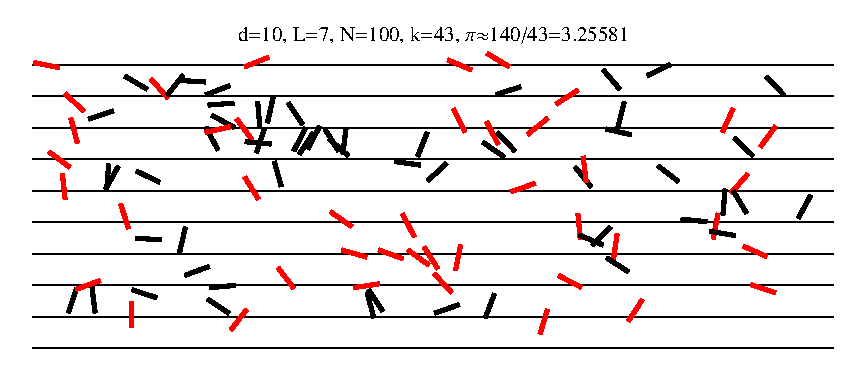
\includegraphics[height=0.3\textheight]{buffonsneedles.eps}
		\caption{Beispiel f"ur eine Realisierung des Buffon--Nadel--Experiments mit 100 geworfenen Nadeln. Der erhaltene Sch"atzwert f"ur $\pi$ ist bei so wenigen Nadeln nicht sehr genau.}
		\label{fig:buffon}
	\end{figure}
	
	\subsection{Das Integrationsproblem}\label{subsec:integrationsproblem}
	Betrachten wir das Integral
	\begin{equation}
		I=\int_\Omega f(x) d\mu(x),
		\label{eq:integration_problem}
	\end{equation}
	wobei $\Omega$ das Integrationsgebiet, $f : \Omega \to \mathbb{R}$ eine reellwertige Funktion und $\mu$ ein Ma"s auf $\Omega$ ist. F"ur die folgende Darstellung nehmen wir an, da"s $$\Omega=[0,1]^d$$ der $d$--dimensionale Einheitsw"urfel und $I_d$ das zugeh"orige Integral ist.
	\subsubsection{Klassische numerische Quadraturverfahren}
	Die klassische numerische Herangehensweise (wenn keine analytische L"osung m"oglich oder praktikabel ist) sind {\em Tensor--Produkt--Verfahren}. Die Idee dabei ist, f"ur jede Dimension ein eindimensionales Quadratur--Verfahren zu w"ahlen (verschiedene oder das gleiche) und diese zu einem mehrdimensionalen Verfahren zu kombinieren. Ein eindimensionales Verfahren stellt eine gewichtete Summe von Funktionswerten an $M$ (vor dem Auswerten der Funktion) festgelegten St"utzstellen dar:
	$${\tilde I}_1=\sum_{i=1}^M w_i\,f(x_i).$$
	Bekannte Vertreter dieser eindimensionalen Quadraturregeln sind z.B. die {\em Newton--Cotes}- und {\em Gauss--Legendre}--Verfahren. Ein hieraus konstruiertes Tensor--Produkt--Verfahren (wobei wir der Einfachheit halber f"ur alle Dimensionen dasselbe eindimensionale Verfahren zugrundelegen) hat dann die Form:
	$${\tilde I}_d^{\,\text{TP}}=\sum_{i_1}^M\cdots\sum_{i_d}^M w_{i_1}w_{i_2}\cdots w_{i_d}f(x_{i_1},\cdots,x_{i_d}).$$
	Aus einem eindimensionalen Verfahren mit $M$ St"utzstellen erhalten wir also ein $d$--dimensionales Verfahren mit $M^d$ St"utzstellen (Siehe Abb. {\ref{fig:tensorproduct}}).
	\begin{figure}
		\centering
		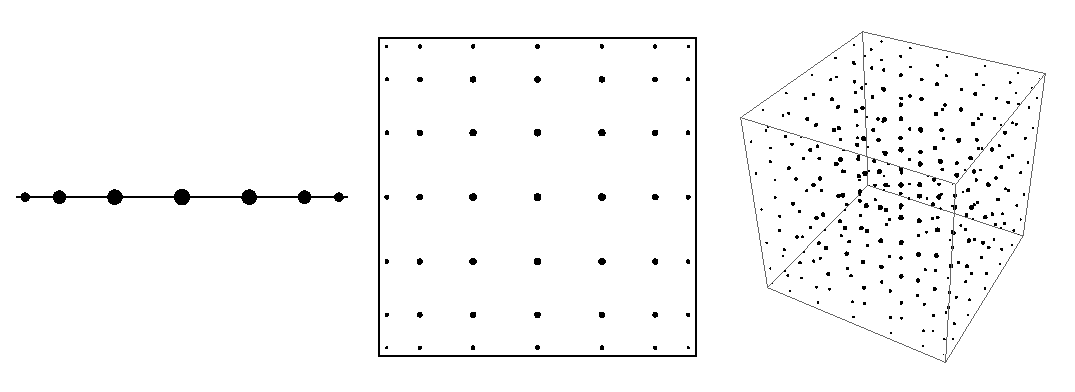
\includegraphics[height=0.25\textheight]{tensorproduct_quadrature.eps}
		\caption{St"utzstellen eines 1D 7--Punkt--Gauss--Legendre--Verfahrens und entsprechender Tensor--Produkt--Verfahren f"ur 2 bzw. 3 Dimensionen. Die Gewichte der St"utzstellen sind durch ihre Gr"o"se kenntlich gemacht.}
		\label{fig:tensorproduct}
	\end{figure}
	
	\subsubsection{einfache Monte--Carlo--Integration}
	Bei der Monte--Carlo--Integration ziehen wir $N$ zuf"allige, gem"a"s einer Wahrscheinlichkeitsdichte $p$ verteilte St"utzstellen $[X_i|i\in\{1,\dots,N\}]$ in $\Omega$ und sch"atzen dann den Wert des Integrals (\ref{eq:integration_problem}) mit
	\begin{equation}
		{\tilde I}_d^{\,\text{MC}}=\frac{1}{N}\sum_{i=0}^{N-1} \frac{f(X_i)}{p(X_i)}
		\label{eq:mc_integral}
	\end{equation}
	ab. Im Falle unseres $d$--dimensionalen Einheitsw"urfels $\Omega=[0,1]^d$ k"onnen wir besipielsweise jede St"utzstelle aus $d$ gleichf"ormig auf dem Einheitsintervall $[0,1]$ verteilten Zufallszahlen $U_i$ durch einfache Tupelbildung
	$$X_i:=(U_{d i},\dots,U_{d(i+1)-1})$$
	gewinnen. Von der Erwartungstreue des Sch"atzers (\ref{eq:mc_integral}) f"ur unser Integral (\ref{eq:integration_problem}) k"onnen wir uns mit \citep[][2.4]{Veach:1997p9136}
	\begin{align*}
		E[{\tilde I}_d^{\,\text{MC}}] &=E\left[\frac{1}{N}\sum_{i=0}^{N-1}\frac{f(X_i)}{p(X_i)}\right] \\
			&= \frac{1}{N}\sum_{i=0}^{N-1}E\left[\frac{f(X_i)}{p(X_i)}\right] \\
			&= \frac{1}{N}\sum_{i=0}^{N-1}\int_\Omega \frac{f(X_i)}{p(X_i)}p(X_i)\,d\mu(x) \\
			&= \int_\Omega f(x)\,d\mu(x)\\
			&= I
	\end{align*}
	leicht "uberzeugen.
	
	\subsubsection{Vergleich von Tensor--Produkt--Verfahren und einfacher Monte--Carlo--Integration}\label{subsec:integrationsproblem_comparison}
	Wir wollen nun die Konvergenzraten der Tensor--Produkt--Verfahren mit der Konvergenzrate des einfachen Monte--Carlo--Sch"atzers (\ref{eq:mc_integral}) vergleichen. Zur Konstruktion eines Vertreters der Tensor--Produkt--Verfahren verwenden wir beispielhaft das Newton--Cotes--Verfahren. In \citep[][3.1.4]{Stoer:2005p10586} wird als Absch"atzung f"ur den Fehler eines Verfahrens $p$--ter Ordnung (d.h. ein Verfahren, das alle Polynome bis zum Grad $p$ exakt integriert) und Schrittweite $h(\approx\frac{b-a}{N}=\mathcal{O}(N^{-1}))$ der St"utzstellen
	\begin{equation}
		\int_a^b P_n(x)-f(x)dx=h^{p+1}K f^{(p)}(\xi),\quad\xi\in(a,b)
		\label{eq:quadrature_error}
	\end{equation}
	angegeben, wobei $n$ die Anzahl der St"utzstellen, $P_n$ das Interpolationspolynom f"ur die St"utzstellen und K eine Konstante ist. Gauss--Legendre--Verfahren sind von der Ordnung $2n-1$, d.h. die Konvergenzrate dieser $n$--Punkt--Formel ist demnach von der Gr"o"senordnung $\mathcal{O}(h^{2n})=\mathcal{O}(N^{-2n})$.\footnote{$N$ bezeichnet die Anzahl der St"utzstellen f"ur das gesamte Integrationsintervall. Der Sch"atzwert f"ur das Integral wird dann durch $\frac{N}{n}$--maliges Anwenden der $n$--Punkt--Formel berechnet}
	Durch Bildund der entsprechenden $d$--dimensionalen Tensor--Produkt--Regel "andert sich die Konvergenzrate in Bezug auf die Schrittweite $h$ nicht. Da unsere $N$ St"utzstellen sich nun aber auf ein $d$--dimensionales Gitter verteilen, teilt sich das Volumen unseres $d$--dimensionalen Einheitsw"urfels in $N$ W"urfel mit einem Volumen von jeweils $h^d$ auf, d.h. f"ur die Schrittweite folgt
	$$\mathcal{O}(1)=V=N h^d \Rightarrow h=\mathcal{O}\left(\left(\frac{1}{N}\right)^{1/d}\right)=\mathcal{O}\left(N^{-1/d}\right)$$	
	und damit f"ur die Konvergenzrate in Bezug auf die Gesamtst"utzstellenzahl
	$$\mathcal{O}(h^{2n})=\mathcal{O}(N^{-2n/d}).$$
	Dies bedeutet, da"s Tensor--Produktverfahren mit steigender Dimension des Integrationsgebietes an Effizienz verlieren. Bei hochdimensionalen Problemen kann dies kaum durch Verfahren h"oherer Ordnung ausgeglichen werden, da Verfahren h"oherer Ordnung, wie oben in (\ref{eq:quadrature_error}) zu sehen auch gr"o"sere Anforderungen an die Glattheit der Funktion stellen. Ausserdem kann die exponentiell steigende Anzahl aller $N \geq n^d$ mindestens n"otigen Funktionsaufrufe zu einem Problem werden. Der Effekt wird bei steigender Dimension und Ordnung des Verfahrens nur noch schlimmer, was ein Ausgleichen der schlechteren Konvergenzrate bei h"oheren Dimensionen durch Erh"ohen der Ordnung des Verfahrens schnell praktisch unm"oglich werden l"asst. Dies wird h"aufig als {\em Curse~of~Dimensionality} (Fluch der Dimensionalit"at) bezeichnet.
	
	Bei der Monte--Carlo--Integration k"onnen wir die Konvergenzrate anhand der Varianz unseres Monte--Carlo--Sch"atzers (\ref{eq:mc_integral}) bestimmen \citep[][2.4.1]{Veach:1997p9136}. Nennen wir der "Ubersicht wegen
	$$Y_i=\frac{f(X_i)}{p(X_i)}$$
	und den MC--Sch"atzer mit $N$ gezogenenen Werten
	$$F_N=\frac{1}{N}\sum_{i=0}^{N-1} Y_i.$$
	Dann gilt f"ur die Varianz eines beliebigen Samples
	\begin{equation}
		V[Y_i]=E[(Y_i-E[Y_i])^2]=E[Y_i^2]-E[Y_i]^2=\int_\Omega \frac{f(x)^2}{p(x)}d\mu(x)-I^2.
		\label{eq:mc_variance}
	\end{equation}
	Da die Werte unabh"angig gezogen sind gilt f"ur die Varianz des Sch"atzer mit $N$ Werten
	$$V[F_N]=V\left[\frac{1}{N}\sum_{i=0}^{N-1}Y_i\right]=\frac{1}{N^2}V\left[\sum_{i=0}^{N-1}Y_i\right]=\frac{1}{N^2}\sum_{i=0}^{N-1}V[Y_i]=\frac{1}{N}V[Y_i],$$
	d.h. die Varianz des Sch"atzers sinkt invers mit der Anzahl $N$ an gezogenen Werten. Daraus folgt sofort die Standardabweichung
	$$\sigma[F_N]=\frac{1}{\sqrt{N}}\sigma[Y_i],$$
	was einer Konvergenzrate von $\mathcal{O}(N^{-1/2})$ entspricht. Die Konvergenzrate des Monte--Carlo--Sch"atzers ist im Gegensatz zur Konvergenzrate der Tensor--Produkt--Verfahren also unabh"angig von der Dimension des Integrationsgebietes, d.h. das Verfahren leidet {\em nicht} unter dem {\em Curse~of~Dimensionality}! Ausserdem mussten wir nirgendwo Bedingungen an die Glattheit der Funktion stellen, was bei Funktionen mit Diskontinuit"aten von Vorteil ist.
	
	Zusammenfassend k"onnen wir also feststellen, da"s Monte--Carlo--Integration bei hochdimensionalen Integrationsproblemen und Funktionen mit Diskontinuit"aten klar gegen"uber klassischen Tensor--Produktverfahren vorzuziehen ist. F"ur niedrigdimensionale ($d\lessapprox 7$) Gebiete mit glatten Integranden sind die klassischen Methoden hingegen besser geeignet.
	
	
	\subsection{Importance--Sampling}
	Wir sind bei unserem MC--Sch"atzer (\ref{eq:mc_integral}) nicht darauf beschr"ankt eine gleich\-f"or\-mi\-ge Wahrscheinlichkeitsdichte $p$ zu w"ahlen. Es kann sogar die Effizienz des Verfahrens betr"achtlich verbessern, wenn wir eine geeignete Wahrscheinlichkeitsdichte $p$ w"ahlen. Schauen wir uns daher die Formel (\ref{eq:mc_variance}) f"ur die Varianz nochmal an, da"s es zu minimieren gilt, um zu verstehen, was ``geeignet'' bedeutet. Nimmt die Wahrscheinlichkeitsdichte beispielsweise die ideale Form
	\begin{equation}
		p(x)=\frac{|f(x)|}{\int_\Omega |f(z)|d\mu(z)}
		\label{eq:ideal_importance_pdf}
	\end{equation}
	an, kann man mit der {\em Jensenschen~Ungleichung} zeigen, da"s dann das Integral in (\ref{eq:mc_variance}) und damit die Varianz insgesamt minimal wird. Nimmt $f$ keine negativen Werte an, verschwindet die Varianz dieses Sch"atzers sogar, da in (\ref{eq:mc_integral}) dann nur noch "uber die konstante L"osung (in Form der Normierungskonstanten) gemittelt wird. Wenn wir das Normierungs--Integral im Nenner von (\ref{eq:ideal_importance_pdf}) l"osen k"onnten, w"are allerdings auch die urspr"ungliche Integration (\ref{eq:integration_problem}) kein Problem! Daher suchen wir in der Praxis nach einem $p$, das m"oglichst "ahnlich zu $|f|$ und gleichzeitig normierbar ist.
	
	
	\subsection{Monte--Carlo--Markov--Chain--Verfahren}
	Bisher sind wir bei unserem Monte--Carlo--Sch"atzer (\ref{eq:mc_integral}) von einer zugrundeliegenden Stichprobe aus $N$ unabh"angigen und identisch gem"a"s $p$ verteilten St"utzstellen ausgegangen, deren zugeh"rige Funktionswerte gemittelt als Sch"atzer f"ur den Wert des Integrals (\ref{eq:integration_problem}) dienen. Wenn wir aber unsere Funktionswerte in jedem Fall mitteln, dann ist die Unabh"angigkeit der gezogenen St"utzstellen nicht relevant, da die Reihenfolge, in der sie gezogen werden, den Mittelwert nicht beeinflusst. Essentiell ist also lediglich, dass sie identisch gem"a"s $p$ verteilt sind.
	
	Diese Freiheit nutzen sogenannte Monte--Carlo--Markov--Chain--Verfahren (MCMC--Verfahren). Sie stellen ein Verfahren dar, um aus einem Zustandsraum $\Omega$ gem"a"s einer gegebenen Wahrscheinlichkeitsdichte $p$ verteilte Werte zu ziehen. Dies wird durch die Konstruktion eines Zufallspfads ({\em random~walk}) im Zustandsraum, dirigiert durch eine Markov--Kette, erreicht. Dabei mu"s sichergestellt werden, da"s die so erzeugten Werte auch gem"a"s $p$ verteilt sind und insbesondere jeder Punkt im Zustandsraum, auf dem $p$ nicht verschwindet, auch erreicht werden kann.
	
	Wie im n"achsten Abschnitt gezeigt wird, ist dies mit erstaunlich wenig Aufwand m"oglich. Die Kombination aus Vielseitigkeit, M"achtigkeit und Einfachheit hat MCMC--Verfahren in vielen Bereichen\footnote{Beispiele finden sich u.a. in der statistischen Physik, in der Finanzmathematik und zur Berechnung von A--posteriori--Wahrscheinlichkeiten in der Bayes'schen Statistik \citep{Geweke:1989p10465}, z.B. mit Anwendungen in der Bioinformatik und Medizin. Weitere interessante und ungew"ohnliche Anwendungen finden sich in \citep{Diaconis:2009p4122}} zu einem Hauptverfahrensbestandteil gemacht.
	
	
	\subsubsection{Metropolis--Hastings--Algorithmus}
	Unter den MCMC--Verfahren ist eines der bekanntesten der {\em Metropolis--Hastings--Algorithmus} (MH), der durch eine Arbeit in der statistischen Physik von \citet{Metropolis:1953p3364} in einer einfachen Form vorgestellt und sp"ater durch \citet{Hastings:1970p3387} verallgemeinert wurde.

	Beim MH--Algorithmus ziehen wir aus einem Zustandsraum $\Omega$ Elemente $x \in \Omega$ gem"a"s der (nicht notwendigerweise normierten!) Wahrscheinlichkeitsdichte $f : \Omega \rightarrow \mathbb{R}_{\geq 0}$. Die Elemente werden dabei mit einem Zufallspfad durch den Zustandsraum generiert. Wir ver"andern dazu den aktuellen Zustand $x$ nach einem frei w"ahlbaren Schema (im Folgenden Mutation genannt) in einen neuen Zustand $x'$.
	Dabei stellen wir folgende Bedingungen an eine Mutation:
	\begin{itemize}
		\item{wenn der "Ubergang vom Zustand $x$ nach $x'$ m"oglich ist, muss auch der "Ubergang zur"uck von $x'$ nach $x$ m"oglich sein}
		\item{es muss jeder Zustand $x \in \Omega$ durch eine Kette von "Uberg"angen erreichbar sein (Ergodizit"at)}
		\item{Die "Ubergangswahrscheinlichkeit $T(x'|x)$ durch unser Mutations--Schema von Zustand $x$ zum Zustand $x'$ zu kommen muss f"ur gegebenes $x$ und $x'$ berechenbar sein}
	\end{itemize}
	Mutationen sind also etwas formaler formuliert bedingte Wahrscheinlichkeitsverteilungen, die durch das Herkunftselements parametrisiert sind, nicht normiert sein m"ussen und f"ur die
	$$\forall x,x'\in\Omega : \quad T(x'|x)>0 \Leftrightarrow T(x|x')>0$$
	wahr ist.
	
	\paragraph{Detailed Balance:}
	Da die Mutation, mit der wir den neuen Zustand generieren, nichts mit der Wahrscheinlichkeitsdichte $f$ zu tun haben mu"s, brauchen wir eine M"oglichkeit die Verteilung der Zust"ande gem"a"s $f$ sicherzustellen.
	Betrachten wir eine gro"se Zahl von gleichartigen aber unabh"angigen Markov--Ketten, die alle mit einer gewissen Wahrscheinlichkeit $p(x'|x)$ vom Zustand $x$ in den Zustand $x'$ "ubergehen, dann ist eine M"oglichkeit eine station"are Zustandsdichte $f$, gemittelt "uber die aktuellen Zust"ande aller Markov--Ketten, zu erreichen, zu verlangen, da"s
	\begin{equation}
		\forall x,x' \in \Omega :\quad f(x)p(x'|x) = f(x')p(x|x')
		\label{eq:dynamic_equlibrium}
	\end{equation}
	({\em =Detailed Balance}) gilt, d.h. da"s die "Ubergangsraten zwischen zwei beliebigen Zust"anden sich im dynamischen Gleichgewicht befinden.
	Da $T$ die "Ubergangswahrscheinlichkeiten aber schon festlegt, behalten wir uns das Recht vor, einen durch Ziehen aus $T$ vorgeschlagenen Zustands"ubergang nur mit der Wahrscheinlichkeit $a(x'|x)$ anzunehmen und ansonsten abzulehnen,	um {\em Detailed Balance} sicherstellen zu k"onnen:
	\begin{equation}
		p(x'|x) = T(x'|x)a(x'|x)
		\label{eq:acceptance_prob_intro}
	\end{equation}
	\begin{equation}
		(\ref{eq:dynamic_equlibrium}) \stackrel{(\ref{eq:acceptance_prob_intro})}{\Longrightarrow}
		\forall x,x' \in \Omega :\quad f(x)T(x'|x)a(x'|x) = f(x')T(x|x')a(x|x')
		\label{eq:detailedbalance}
	\end{equation}
	Dies l"asst noch immer verschiedene M"oglichkeiten zu, die Akzeptanzwahrscheinlichkeit zu bestimmen. Eine effiziente und dadurch beliebte Wahl ist dabei Folgende: ist $f(x')>f(x)$ nehmen wir den neuen Zustand auf jeden Fall an, ansonsten mit der Wahrscheinlichkeit $(f(x')T(x|x'))/(f(x)T(x'|x))$. Dies l"asst sich zusammenfassen zu
	\begin{equation}
		a(x'|x)=\text{min}\left(1,\frac{f(x')T(x|x')}{f(x)T(x'|x)}\right)
		\label{eq:acceptanceratio}
	\end{equation}
	
	
	\paragraph{Pseudocode:}
	In Pseudocode sieht der Algorithmus dann wie folgt aus:
	\begin{algorithmic}
		\STATE $x_1 \leftarrow$ Anfangszustand
		\FOR{$i=1$ to $N$}
			\STATE ziehe $x'$ gem"a"s $T(x'|x_i)$
			\STATE $a(x'|x_i) \leftarrow \text{min}\left(1, \frac{f(x')T(x|x')}{f(x)T(x'|x)}\right)$
			\STATE $u\leftarrow$ Zufallszahl aus $[0,1]$
			\IF{$u < a(x'|x_i)$}	\STATE $x_{i+1}=x'$
			\ELSE	\STATE $x_{i+1}=x_i$
			\ENDIF
	  \ENDFOR
	\end{algorithmic}
	Als Ergebnis erhalten wir eine Liste von Samples, die gem"a"s $f$ verteilt sind. Die Samples sind allerdings nicht unabh"angig, sondern im Gegenteil h"aufig hochkorreliert. Wenn wir nur an statistischen Kenngr"o"sen wie dem Mittelwert oder der Varianz einer Stichprobe interessiert sind ist die Korrelation aber irrelevant und stellt somit f"ur uns kein Problem dar. Die Tatsache, da"s die Normierung von $f$ f"ur die Funktion des Verfahrens nicht notwendig ist, bedeutet allerdings auch, da"s wir uns bei Bedarf eine Normierung auf andere Weise beschaffen m"ussen.
	
	
	\subsubsection{Generalisierter Metropolis--Hastings--Algorithmus}
	TODO: Robuste MH--Variante

	\section{Monte--Carlo--Strahlungstransport}
	\subsection{Pfadgenerierung}
	\subsubsection{Raycasting}
	\subsubsection{Distanzsampler}
	TODO: uniform depth sampler, uniform attenuation sampler, enforced uniform attenuation sampler
	
	TODO: Pfadgenerierung, Sch"atzer
